% ======================================================================
%  ClassRoomSTORM Studio V1.2: User Help
%  Self-contained LaTeX source. Compile from this directory with:
%      pdflatex ClassRoomSTORM_Help.tex   (run twice)
%  Figures live in ../figures/help/ and ../figures/theory/.
%  Screenshot placeholders (\figph) are to be replaced with
%  \includegraphics once the application screenshots are captured.
% ======================================================================
\documentclass[11pt,a4paper]{article}

\usepackage[utf8]{inputenc}
\usepackage[T1]{fontenc}
\usepackage{lmodern}
\usepackage{amsmath,amssymb}
\usepackage{geometry}
\usepackage{graphicx}
\usepackage[font=small,labelfont=bf]{caption}
\usepackage{booktabs}
\usepackage{tabularx}
\usepackage{enumitem}
\usepackage{needspace}
\usepackage{xcolor}
\usepackage{tcolorbox}
\tcbuselibrary{breakable}
\usepackage{hyperref}
\usepackage{cleveref}

\geometry{margin=24mm}
% Keep figure-only pages aligned at the top with a deliberate inter-float gap.
\makeatletter
\setlength{\@fptop}{0pt}
\setlength{\@fpsep}{16pt plus 2pt minus 2pt}
\setlength{\@fpbot}{0pt plus 1fil}
\makeatother
\graphicspath{{../figures/help/}{../figures/theory/}{figures/help/}{figures/theory/}}
\hypersetup{colorlinks=true, linkcolor=blue!45!black, urlcolor=blue!45!black,
  citecolor=blue!45!black,
  pdftitle={ClassRoomSTORM Studio V1.2: User Help},
  pdfauthor={Awanish Pratap Singh},
  pdfsubject={User guide for the ClassRoomSTORM Studio teaching application}}
\setlist[itemize]{itemsep=2pt, topsep=4pt}
\setlist[enumerate]{itemsep=3pt, topsep=4pt}
\emergencystretch=3em

% ---- Callout boxes --------------------------------------------------
\newtcolorbox{csnote}[1][Note]{breakable, colback=blue!4, colframe=blue!55!black,
  fonttitle=\bfseries, coltitle=white, title={#1}, boxrule=0.5pt, arc=2pt}
\newtcolorbox{cstip}[1][Tip]{breakable, colback=green!6, colframe=green!45!black,
  fonttitle=\bfseries, coltitle=white, title={#1}, boxrule=0.5pt, arc=2pt}
\newtcolorbox{cswarn}[1][Warning]{breakable, colback=red!5, colframe=red!60!black,
  fonttitle=\bfseries, coltitle=white, title={#1}, boxrule=0.5pt, arc=2pt}

% ---- Screenshot placeholder (for application screenshots only) ------
\newcommand{\figph}[2][6cm]{%
  \begingroup
  \setlength{\fboxsep}{8pt}\setlength{\fboxrule}{0.6pt}%
  \fcolorbox{gray!55}{gray!8}{%
    \parbox[c][#1][c]{\dimexpr\linewidth-2\fboxsep-2\fboxrule\relax}{%
      \centering\itshape\small #2\par\medskip
      \upshape\footnotesize\textcolor{gray!60!black}{[\,screenshot placeholder: capture from the running application\,]}}}%
  \endgroup}

\newcommand{\ui}[1]{\textbf{#1}}
\newcommand{\file}[1]{\texttt{#1}}
\newcommand{\app}{ClassRoomSTORM}
\newcommand{\studio}{\app{} Studio}

\title{\textbf{\studio{} V1.2}\\[2pt]\large User Help: Virtual and Experimental
       Super-Resolution Microscopy}
\author{Awanish Pratap Singh}
\date{Software version 1.2}

% ======================================================================
\begin{document}
\maketitle
\thispagestyle{empty}

\begin{abstract}
\noindent This Help document explains how to install and use \studio{} V1.2, a
desktop teaching application for localization-based super-resolution microscopy.
It describes the tasks you can perform and explains each screen and control. The physics
behind the method (diffraction, blinking, localization, and precision) is
explained in the companion document, \emph{\app{} Theory Notes}.
\end{abstract}

\begingroup\small\tableofcontents\endgroup
\newpage

% ======================================================================
\section{What \app{} Is and Is Not}
\label{sec:what}

\studio{} V1.2 is a desktop teaching application for \emph{localization-based
super-resolution microscopy}. It has two workflows:

\begin{itemize}
  \item the \textbf{Virtual Experiment}, which creates synthetic ``blinking''
        videos from a pattern of points; and
  \item \textbf{SR Reconstruction}, which turns a blinking video into a sharper
        \emph{reconstructed image} by locating individual bright spots frame by
        frame and accumulating their positions.
\end{itemize}

\app{} reproduces the \emph{statistical and computational logic} of
single-molecule localization microscopy (SMLM), the family of methods that includes STORM and PALM, in a form that needs no lasers, no fluorescence
optics, and no scientific camera.

\begin{csnote}[What this means]
\app{} is a \emph{learning tool}, not a fluorescence microscope and not a
research-grade analysis package. Its reconstruction deliberately uses a simple method that detects bright spots, calculates an intensity-weighted centroid, and accumulates the positions, so that students can inspect and understand every step. It
does not perform Gaussian model fitting, maximum-likelihood estimation,
or drift correction. Manual physical calibration is applied to exported
coordinates; it does not estimate uncertainty (see the \emph{Theory} document).
\end{csnote}

% ======================================================================
\section{Concepts in 60 Seconds}
\label{sec:concepts}

\begin{description}[style=unboxed, leftmargin=0pt]
  \item[Blinking video.] A video with many frames in which, at any instant, only
        a few light sources (``blinkers'') are switched on. Each blinker appears
        as a small blurred spot.
  \item[Localize.] In each frame, \app{} finds the centre of every bright spot.
        Although the spot is blurry and several pixels wide, its \emph{centre}
        can be estimated to better than one pixel.
  \item[Accumulate.] The centres found in all frames are collected into a single image, the \emph{reconstructed image}. Because it is built from sharp
        centres rather than blurry spots, it is much crisper than the raw video.
  \item[Compare.] The arithmetic mean of the video frames (\ui{Raw Mean}) is
        blurry; the \ui{Super-Resolution} image is the accumulated
        reconstruction. Comparing the two is the central activity.
\end{description}

\begin{figure}[htbp]
  \centering
  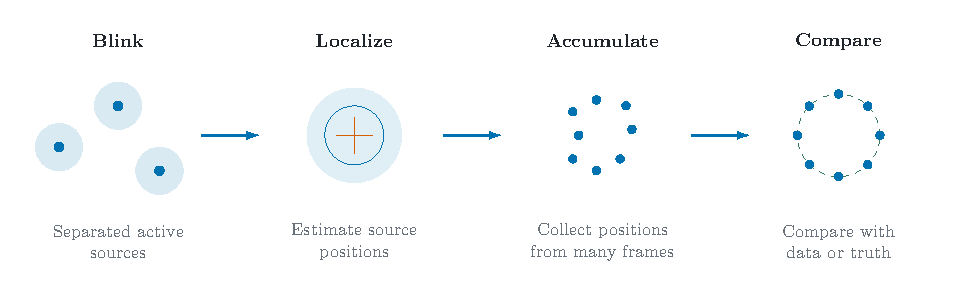
\includegraphics[width=\linewidth]{H1_concept_loop}
  \caption{Conceptual progression from sparse blinking through position estimation to comparison with data or known truth.}
  \label{fig:loop}
\end{figure}

\begin{cstip}[The truth-data rule]
When you create a Virtual Experiment, \app{} also saves the exact positions it
used, in a file called \file{truth.csv}. Reconstruction does \emph{not} read this
file. You compare your reconstruction against it only \emph{afterwards}, to evaluate your result, much as you would check an answer key after solving a problem. Keep \file{truth.csv} in its
original folder and do not feed it into the reconstruction.
\end{cstip}

% ======================================================================
\section{Installation and Setup}
\label{sec:install}

\app{} V1.2 is a Python desktop application. The user package includes ready-made
setup and launch scripts, so most users never need to type any commands.

\paragraph{Requirements.} The Windows setup script looks for Python 3.11, 3.12,
or 3.13 automatically, using the Python launcher (\file{py}) when available. If
no supported Python is found, it can offer to install Python 3.11 with
\file{winget} or open the official Python download page. On macOS, install
Python 3.10 or newer from \url{https://www.python.org/} before running setup.
First-time setup downloads roughly 250-350~MB of packages from the Python
Package Index (PyPI), so an internet connection is needed unless your package
includes an offline \file{wheels} folder (see below).

\paragraph{Recommended: run the setup script.}
\begin{itemize}
  \item \textbf{Windows:} double-click \file{setup\_windows.bat}.
  \item \textbf{macOS:} double-click \file{setup\_macos.command}. The first time,
        macOS may block it; right-click the file and choose \ui{Open}, or run
        \file{chmod +x setup\_macos.command} in Terminal once.
\end{itemize}
The script builds a private environment (a \file{.venv} folder inside the package)
and installs the required packages. When it finishes, it prints
\emph{Setup completed}. If it fails partway through, it preserves the environment for a
retry. The launcher checks required imports before starting.

\paragraph{Offline installation.} If the package folder contains a \file{wheels}
folder, the setup script installs from it automatically and no internet access is
needed. This is useful on restricted or proxy-protected networks.

\paragraph{Manual installation (advanced).} Instead of using the script, you may open a
terminal in the package folder and run \file{python -m venv .venv}, activate it
(Windows PowerShell activation command shown below;
macOS or Linux: \file{source .venv/bin/activate}), and then run
\file{python -m pip install -{}-upgrade pip} followed by
\file{python -m pip install -r requirements.txt}. The standard packages are
\file{numpy}, \file{opencv-python}, \file{matplotlib}, \file{Pillow}, and
\file{PySide6}.
\begin{quote}\small\ttfamily
.{\textbackslash}.venv{\textbackslash}Scripts{\textbackslash}Activate.ps1
\end{quote}

\begin{csnote}[Optional extras]
\textbf{Graphviz} produces cleaner pipeline diagrams. Without it, \app{} draws
the same diagrams with Matplotlib instead, so Graphviz is not required. \textbf{NVIDIA
CUDA GPU} acceleration is experimental; install it with
\file{python -m pip install -r requirements-gpu.txt} only if you have a
CUDA-capable NVIDIA card. AMD, Intel, and Apple Silicon GPUs are not supported in
V1.2; those systems use the CPU.
\end{csnote}

% ======================================================================
\section{Starting \studio{}}
\label{sec:launcher}

Start the application with the launch script in the package folder:
\begin{itemize}
\item \textbf{Windows}: double-click \file{launch\_studio\_windows.bat}.
\item \textbf{macOS}: double-click \file{launch\_studio\_macos.command}.
\end{itemize}
The launch
script checks that the required packages are installed and, if they are missing,
asks you to run the setup script first. Advanced users may instead run
\file{python apps/ClassRoomSTORM\_Studio.py} from an activated environment.

The \studio{} launcher window offers two large buttons:
\begin{itemize}
  \item \ui{Virtual Experiment}: create blinking data from a logo, letter, or
        pattern (\cref{sec:virtual});
  \item \ui{SR Reconstruction}: reconstruct a recorded or simulated blinking
        video (\cref{sec:recon}).
\end{itemize}
Two text links, \ui{Help} and \ui{Theory}, open this document and the Theory
companion (the PDF files in the \file{docs} folder).

\begin{cswarn}[The launcher closes when you open a workflow]
When you click \ui{Virtual Experiment} or \ui{SR Reconstruction}, the launcher
window fades out and \emph{closes itself}; the chosen workflow then opens as a
separate window. This is normal; the application has not crashed. To return to
the launcher, use the \ui{Back to Studio} toolbar button at the top of the
workflow window, or run the launch command again.
\end{cswarn}

\begin{figure}[htbp]
  \centering
  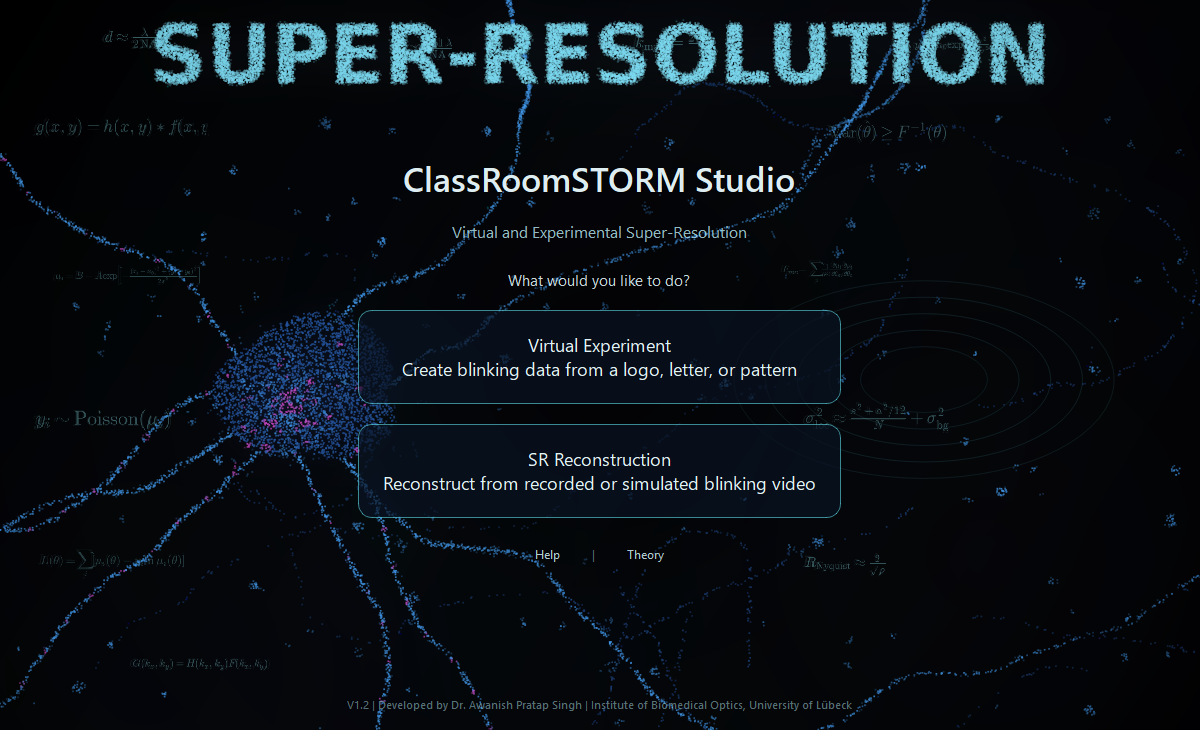
\includegraphics[width=0.90\linewidth]{H2_launcher_screenshot}
  \caption{The \studio{} launcher: the two workflow buttons
  (\ui{Virtual Experiment}, \ui{SR Reconstruction}) and the \ui{Help} and
  \ui{Theory} links, over the animated localization background.}
  \label{fig:launcher}
\end{figure}

% ======================================================================
\section{Quick Start: First Virtual Experiment and Reconstruction}
\label{sec:quickstart}

This walkthrough takes about ten minutes and uses only simulated data.

\begin{enumerate}
  \item \textbf{Launch} the Studio and click \ui{Virtual Experiment}.
  \item On the \ui{1 Pattern} page, set \ui{Pattern} to \texttt{text} and type a
        short word (for example, \texttt{ABBE}) in the \ui{Text} box.
  \item On the \ui{2 Blinking} page, set \ui{Frames} to about \texttt{300} for a
        quick first run.
  \item On the \ui{3 Image Formation} page, keep the default settings.
  \item On the \ui{4 Preview} page, click \ui{Preview Source Mask} and then
        \ui{Preview Sample Blink Frame} to see what you are about to generate.
  \item On the \ui{5 Export} page, click \ui{Export Dataset}. Note the output
        folder shown; it now contains \file{blinking\_video.mp4}.
  \item \textbf{Relaunch} the Studio (it closed in step~1) and click
        \ui{SR Reconstruction}.
  \item On the \ui{1 Load Video} page, click \ui{Browse Video} and select the
        \file{blinking\_video.mp4} you just created. The first frame appears.
  \item Leave \ui{Blinker mode} on \texttt{auto} and \ui{Processing backend} on
        \ui{Serial}. On the \ui{6 Results} page, click \ui{Run Reconstruction}.
  \item Open \ui{Main Results}, then the \ui{Linked Profiles} tab. Click on a
        bright part of the image and compare the wide red curve (raw) with the
        narrow blue curve (reconstruction).
\end{enumerate}

\begin{figure}[htbp]
  \centering
  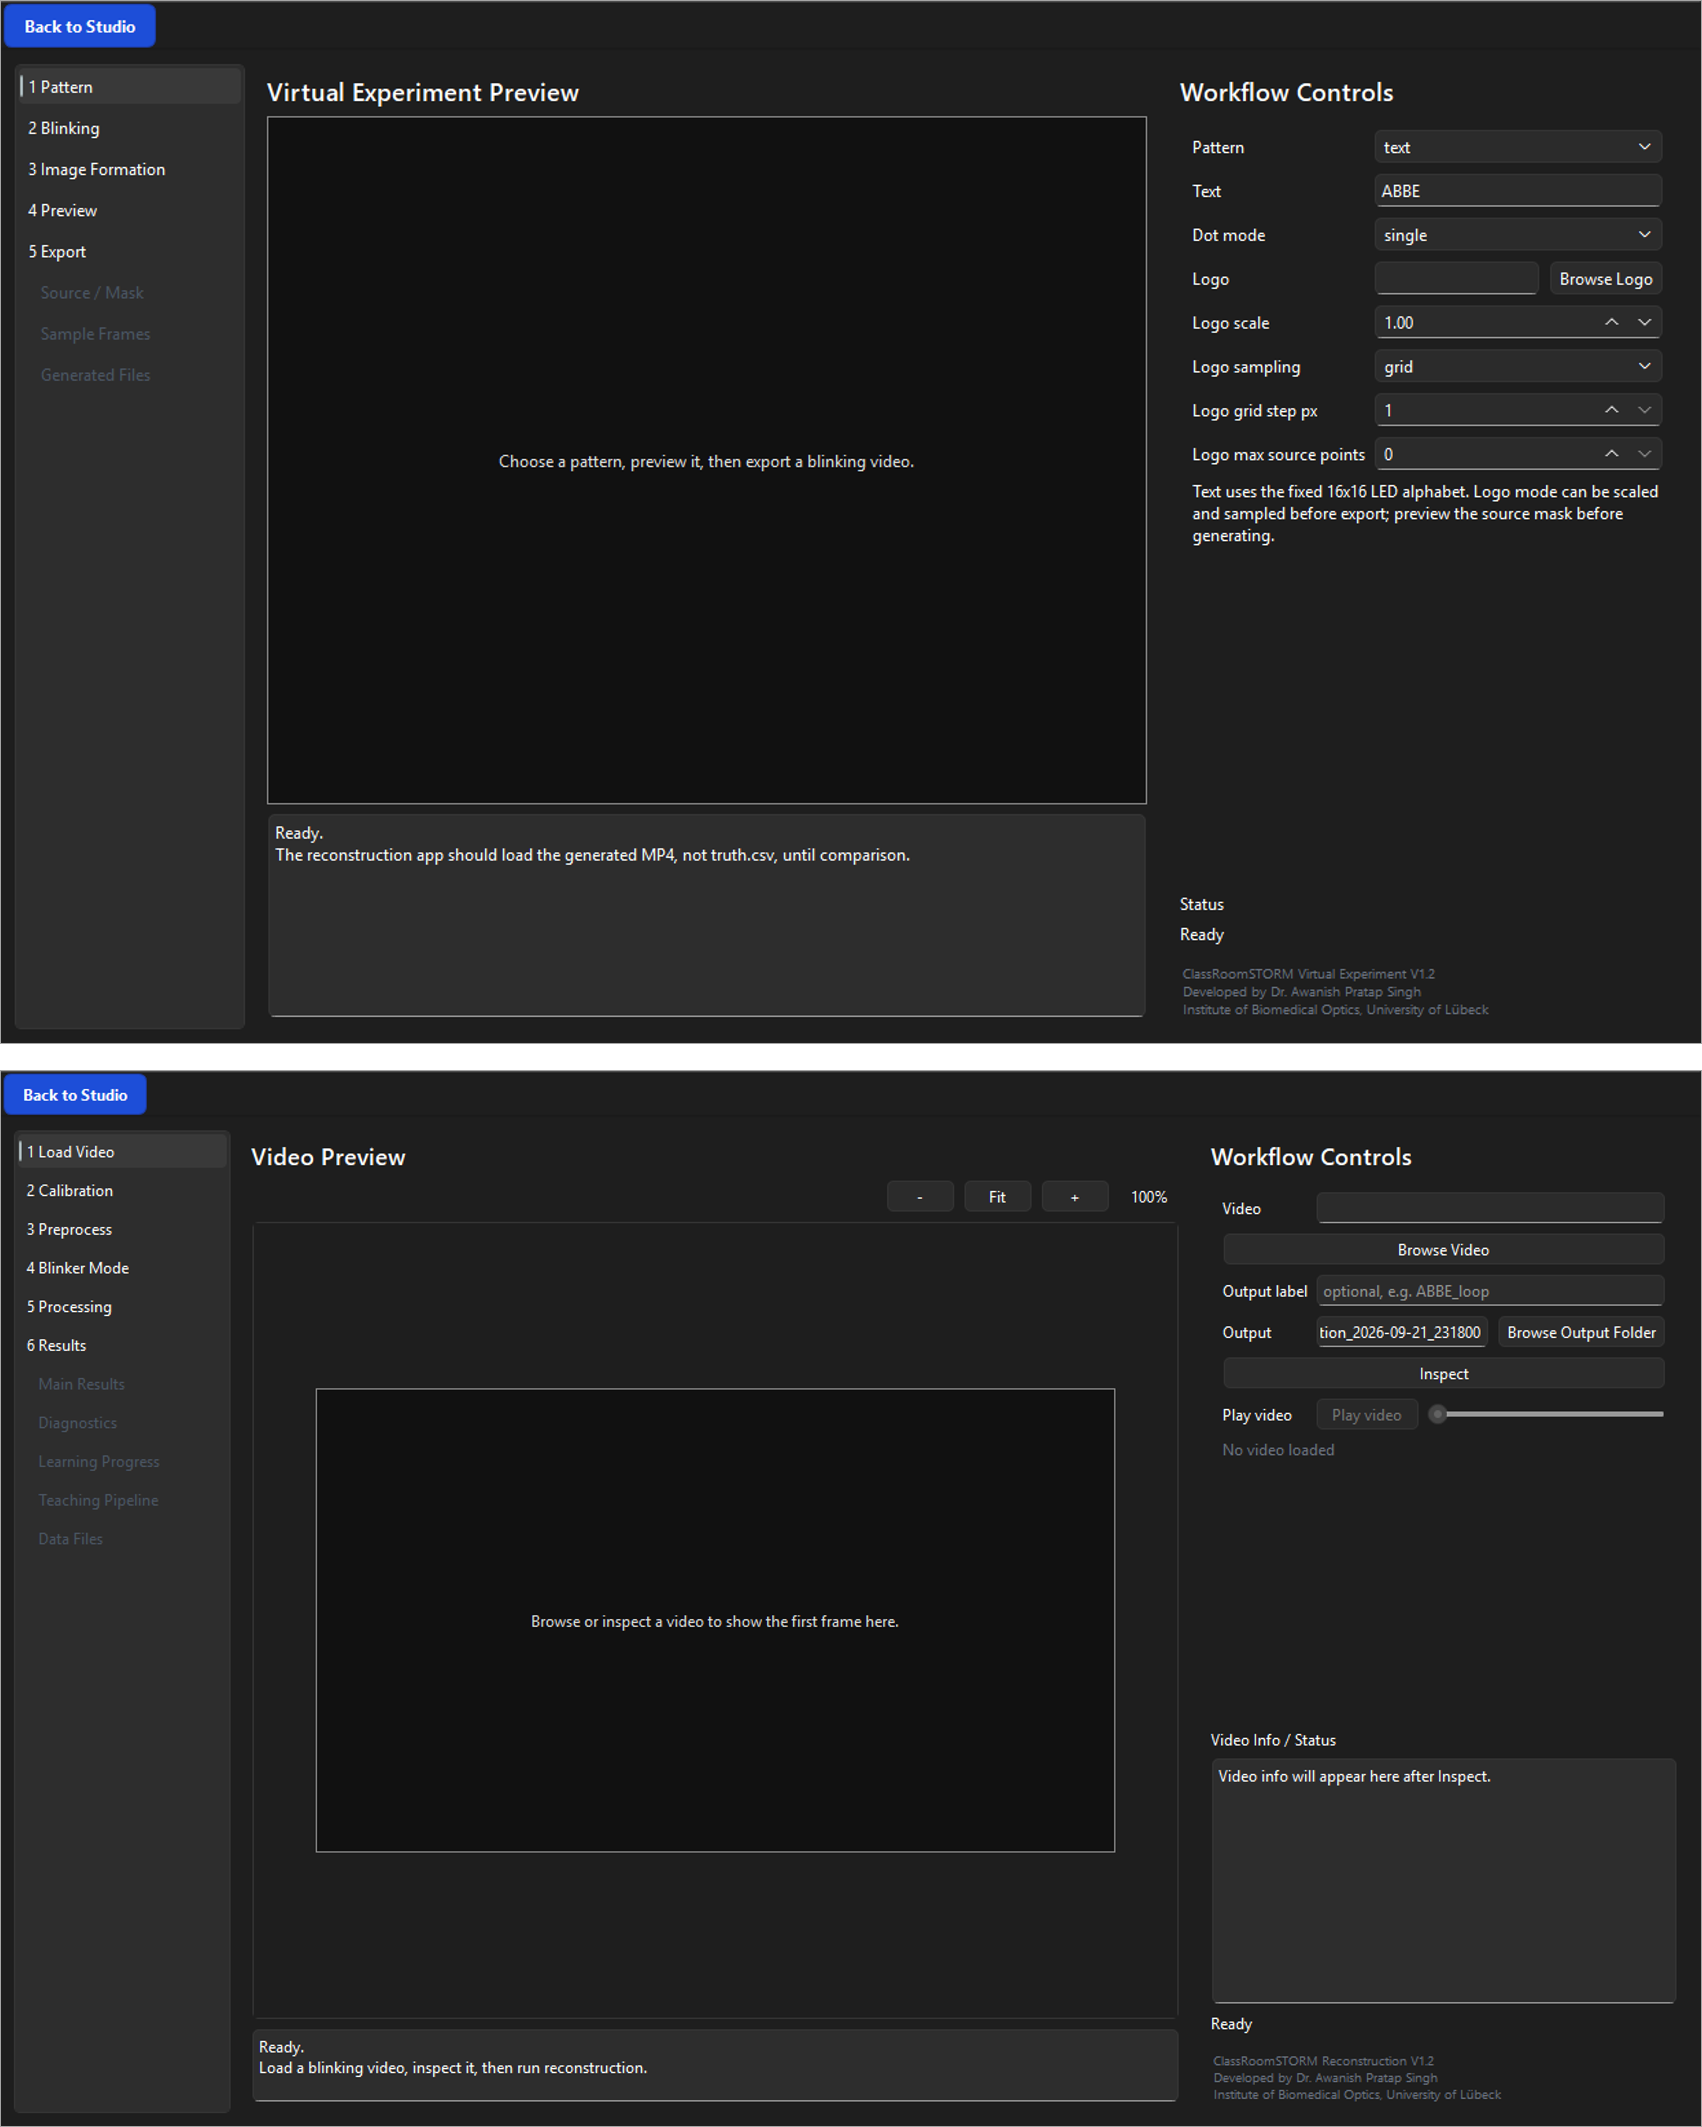
\includegraphics[width=\linewidth]{H3_quickstart_montage}
  \caption{The two workflow windows used in the Quick Start: the Virtual
  Experiment (top) and SR Reconstruction (bottom).}
  \label{fig:quickstart}
\end{figure}

% ======================================================================
\section{Virtual Experiment Step by Step}
\label{sec:virtual}

The Virtual Experiment builds a synthetic blinking video. Its window has five
numbered steps in the left-hand list: \ui{1 Pattern}, \ui{2 Blinking},
\ui{3 Image Formation}, \ui{4 Preview}, and \ui{5 Export}.

\subsection{Step 1: Pattern}
\label{sec:ve-pattern}

The pattern defines \emph{where} the source points are located. Choose one of three
pattern types with the \ui{Pattern} control.

\begin{table}[htbp]
\centering\small
\begin{tabularx}{\linewidth}{@{}lXl@{}}
\toprule
\textbf{Control} & \textbf{What it does} & \textbf{Default}\\
\midrule
\ui{Pattern} & Source pattern type: \texttt{text}, \texttt{dots}, or
  \texttt{logo}. & \texttt{text}\\
\ui{Text} & The word drawn in \texttt{text} mode, using a fixed
  16$\times$16 LED-style alphabet (A-Z, 0-9, space, \texttt{-}, \texttt{\_}).
  & \texttt{ABBE}\\
\ui{Dot mode} & For \texttt{dots} mode: \texttt{single} (one point),
  \texttt{pair} (two close points), or \texttt{random} (several points).
  & \texttt{single}\\
\ui{Logo} & For \texttt{logo} mode: an image file (use \ui{Browse Logo}). The
  image is converted to a black-and-white mask. & -\\
\ui{Logo scale} & Scales the logo mask (0.1-5.0). & \texttt{1.0}\\
\ui{Logo sampling} & How logo pixels become source points: \texttt{grid},
  \texttt{all\_pixels}, or \texttt{random\_max\_points}. & \texttt{grid}\\
\ui{Logo grid step px} & Spacing of the sampling grid, in pixels (1-100).
  & \texttt{1}\\
\ui{Logo max source points} & Upper limit on logo points; \texttt{0} means no
  limit. & \texttt{0}\\
\bottomrule
\end{tabularx}
\caption{Controls on the \ui{1 Pattern} page.}
\label{tab:ve-pattern}
\end{table}

\begin{figure}[htbp]
  \centering
  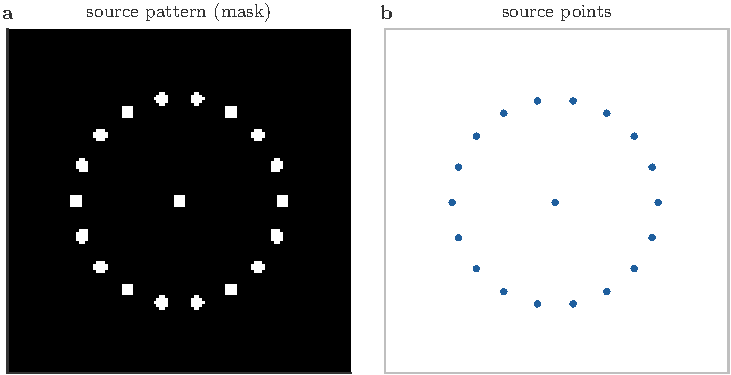
\includegraphics[width=0.80\linewidth]{H4_pattern_preview}
  \caption{A schematic source pattern and one illustrative set of source positions. The mask defines eligible regions; it is not a measured optical image or a guarantee of one emitter per bright connected region.}
  \label{fig:ve-pattern}
\end{figure}

\subsection{Step 2: Blinking}
\label{sec:ve-blinking}

This page controls \emph{how the source points switch on and off} over the
frames of the video.

\begin{table}[htbp]
\centering\small
\begin{tabularx}{\linewidth}{@{}lXl@{}}
\toprule
\textbf{Control} & \textbf{What it does} & \textbf{Default}\\
\midrule
\ui{Frames} & Number of frames in the generated video (1-10000). More frames give a denser reconstruction but require more processing time. & \texttt{1000}\\
\ui{Max blinkers/frame} & The largest number of source points allowed to be on
  in any one frame. The actual number may be lower if spacing rules cannot be
  met. & \texttt{30}\\
\ui{Blinker spacing} & How far apart blinkers that are on simultaneously must be:
  \texttt{separated}, \texttt{touching}, \texttt{overlapping}, or
  \texttt{random}. & \texttt{separated}\\
\ui{Manual min distance px} & A reference separation distance, in pixels, that
  the spacing mode scales. & \texttt{100.0}\\
\ui{Effective min distance} & Read-only. Shows the separation actually applied.
  & -\\
\bottomrule
\end{tabularx}
\caption{Controls on the \ui{2 Blinking} page.}
\label{tab:ve-blinking}
\end{table}

\begin{csnote}[Why blinkers must be separated]
If too many blinkers are on at once and they are close together, their blurred
spots overlap and cannot be distinguished. Sparse, well-separated blinking is what
makes localization possible; this is the core idea of the method (see the
\emph{Theory} document).
\end{csnote}

\subsection{Step 3: Image Formation}
\label{sec:ve-formation}

This page controls the blur, brightness, and noise used to render each source point in a simulated camera image. \Cref{fig:ve-frame} shows one resulting
frame.

\begin{table}[htbp]
\centering\small
\begin{tabularx}{\linewidth}{@{}lXl@{}}
\toprule
\textbf{Control} & \textbf{What it does} & \textbf{Default}\\
\midrule
\ui{sigma\_px} & The blur width $\sigma$ of each spot, in pixels, or the point-spread width (0.5-50). Larger values give wider, blurrier spots.
  & \texttt{10.0}\\
\ui{Spacing px} & The distance, in pixels, between neighbouring points of the
  source mask when they are placed in the image (1-100). & \texttt{2.6}\\
\ui{Brightness} & The base number of signal photons per blinker
  (1-1\,000\,000). & \texttt{80000}\\
\ui{Effective brightness} & Read-only. The brightness actually used (see the
  note below). & -\\
\ui{Background} & A constant background level added to every pixel. &
  \texttt{1.0}\\
\ui{Read noise} & The strength of the camera-like random read noise. &
  \texttt{0.2}\\
\bottomrule
\end{tabularx}
\caption{Controls on the \ui{3 Image Formation} page.}
\label{tab:ve-formation}
\end{table}

\begin{csnote}[\ui{Brightness} vs.\ \ui{Effective brightness}]
\app{} scales the \ui{Brightness} you enter by a factor that grows with the
number of blinkers per frame, so that frames with many blinkers remain visible. The scaled value
is shown in the read-only \ui{Effective brightness} field, and \emph{that} value is used to render the frames. If your frames look brighter or dimmer than
expected, check \ui{Effective brightness}, not \ui{Brightness}.
\end{csnote}

\begin{figure}[htbp]
  \centering
  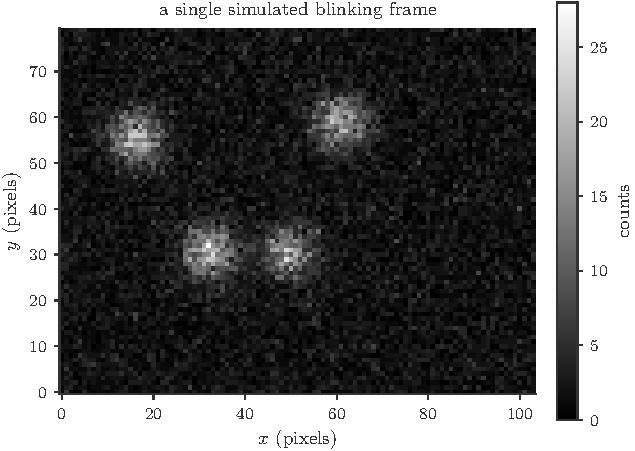
\includegraphics[width=0.70\linewidth]{H5_blinking_frame}
  \caption{One raw synthetic frame from the recorded two-source run. Only one emitter is active in this frame; signal and background are Poisson-distributed.}
  \label{fig:ve-frame}
\end{figure}

\subsection{Step 4: Preview}
\label{sec:ve-preview}

Two buttons let you check your settings before generating the dataset:
\ui{Preview Source Mask} shows the pattern of source points, and \ui{Preview
Sample Blink Frame} shows one example frame. Previewing does not write any files.

\subsection{Step 5: Export}
\label{sec:ve-export}

Choose an output folder (or accept the suggested one) and click
\ui{Export Dataset}. \app{} writes the files listed in \cref{tab:ve-outputs}
and then shows them in the result browser.

The \ui{Frame backend} setting controls how virtual frames are rendered.
\ui{Auto CPU} is the recommended default. \ui{CPU parallel} uses CPU workers,
and \ui{GPU CUDA} is experimental and requires PyTorch CUDA from
\file{requirements-gpu.txt}. If CUDA is unavailable, \app{} falls back to CPU
generation and records the reason in \file{metadata.json}.

The \ui{CPU workers (0=auto)} setting controls CPU frame rendering. Use
\texttt{0} to let \app{} use up to about 90\% of available CPU workers,
\texttt{1} for serial generation, or a larger value to limit CPU-parallel
generation manually.

\begin{table}[htbp]
\centering\small
\begin{tabularx}{\linewidth}{@{}lX@{}}
\toprule
\textbf{File} & \textbf{Contents}\\
\midrule
\file{blinking\_video.mp4} & The blinking video, which is the input for reconstruction.\\
\file{truth.csv} & The exact source positions used. For comparison
  \emph{after} reconstruction only (see the truth-data rule).\\
\file{preview\_frame.png} & A sample blinking frame.\\
\file{pattern\_mask.png} & The source-point mask.\\
\file{metadata.json} & All generation settings.\\
\bottomrule
\end{tabularx}
\caption{Files written by the Virtual Experiment.}
\label{tab:ve-outputs}
\end{table}

% ======================================================================
\section{SR Reconstruction Step by Step}
\label{sec:recon}

SR Reconstruction turns a blinking video into a reconstructed image. The video
may be one you made with the Virtual Experiment or a recorded video of physical blinking sources. The window has six numbered steps: \ui{1 Load Video}, \ui{2 Calibration},
\ui{3 Preprocess}, \ui{4 Blinker Mode}, \ui{5 Processing}, and \ui{6 Results}.

\subsection{Step 1: Load Video}
\label{sec:rc-load}

Click \ui{Browse Video} and choose an MP4, AVI, or MOV file. \app{} reads the
video and shows its first frame and basic information (size, frame count, frame
rate). You may also set an \ui{Output label} and an \ui{Output} folder for the
results. The \ui{Inspect} button repeats this inspection at any time.

The \ui{Play video} button plays the loaded video frame by frame in the
preview, and the slider beside it scrubs through the frames, providing a quick way to
see the raw blinking data before reconstructing it.

\subsection{Step 2: Calibration}
\label{sec:rc-calib}

\begin{csnote}[Calibration applies to exported coordinates]
Choose \ui{Manual calibration}, enter a positive \ui{Unit per pixel}, and set
the \ui{Unit label}, for example, mm. The CSV retains crop-local
\file{x\_px}/\file{y\_px}, adds original-frame
\file{x\_full\_px}/\file{y\_full\_px}, and exports
\file{x\_calibrated}/\file{y\_calibrated} relative to the original frame origin.
Images and linked profiles retain pixel axes. Leave \ui{Pixels only} selected
when a physical scale is unavailable. Calibration does not establish precision.
\end{csnote}

\subsection{Step 3: Preprocess}
\label{sec:rc-preprocess}

If you only want to reconstruct part of the field of view, tick \ui{Enable crop}
and set \ui{Crop x}, \ui{Crop y}, \ui{Crop width}, and \ui{Crop height}. A
rectangle appears on the first-frame preview; \ui{Show crop overlay} and
\ui{Preview cropped region} let you check it.

\begin{cswarn}[Set the crop size before running]
\ui{Crop width} and \ui{Crop height} start at \texttt{0}. If you enable cropping
but leave them at zero, reconstruction stops with an error. Inspecting a video
fills these boxes with the full video size automatically; adjust them from
there.
\end{cswarn}

\begin{csnote}[Background subtraction and threshold]
\ui{Subtract frame median background} subtracts the median intensity of each
cropped frame and clips negative values to zero before thresholding and
localization. This option is off by default and assumes sparse bright emitters on a
roughly uniform background. The exported raw mean remains uncorrected.
\ui{Threshold quantile} defaults to 0.995. Blank and constant frames produce
no localizations; invalid image arrays stop processing with an error.
\end{csnote}

\subsection{Step 4: Blinker Mode}
\label{sec:rc-mode}

The \ui{Blinker mode} control tells \app{} how many bright spots to expect in
each frame:

\begin{description}[style=unboxed,leftmargin=0pt]
  \item[\texttt{single}] At most one localization per frame, from the single brightest region.
  \item[\texttt{multiple}] Several localizations per frame, with each separated bright region located independently.
  \item[\texttt{auto}] \app{} scans the first part of the video and chooses
        \texttt{single} or \texttt{multiple} for you. This is the default.
\end{description}

\begin{cstip}
Use \texttt{single} for data with one blinker at a time, and \texttt{multiple}
when several well-separated blinkers can be on together. If you are unsure, leave the mode on \texttt{auto}. The mode actually used is recorded in \file{summary.json}.
\end{cstip}

\subsection{Step 5: Processing}
\label{sec:rc-processing}

The \ui{Processing backend} controls how the computation is distributed.

\begin{table}[htbp]
\centering\small
\begin{tabularx}{\linewidth}{@{}lX@{}}
\toprule
\textbf{Backend} & \textbf{What it does}\\
\midrule
\ui{Serial} & Processes frames one at a time on the CPU. Simplest and most
  predictable; the recommended starting choice.\\
\ui{Auto CPU} & Uses several CPU cores in parallel when that is worthwhile,
  capped at about 90\% of available CPUs.\\
\ui{Only GPU} & Uses an NVIDIA CUDA GPU for the single-blinker path.\\
\ui{Auto CPU+GPU} & Uses the GPU for single blinkers and parallel CPU processing for multiple blinkers.\\
\ui{Auto CPU+GPU acceleration} & An experimental hybrid path.\\
\bottomrule
\end{tabularx}
\caption{Processing-backend options.}
\label{tab:backends}
\end{table}

\ui{Workers (0=auto)} sets the number of CPU processes; \texttt{0} lets \app{}
choose up to about 90\% of available CPUs. \ui{Max frames (0=all)} limits how
many frames are processed, which is useful for a quick test run.

\begin{cswarn}[GPU backends fall back to the CPU silently]
The GPU backends need an NVIDIA card with CUDA and the optional GPU packages
installed. If the required hardware or packages are missing, \app{} does \emph{not} stop; it quietly runs
on the CPU and records the fallback in \file{summary.json}. If GPU speed
matters, open \file{summary.json} after the run and confirm that the GPU was used.
\end{cswarn}

\subsection{Step 6: Run and Results}
\label{sec:rc-results}

Reconstruction and figure export run in a background worker, so the window
remains responsive. Wait for completion before closing the application.
Choose an empty output folder: existing results are protected from replacement.
When truth comparison is selected, \ui{Truth match radius (px)} sets the maximum
allowed distance. Matching is one-to-one within the same frame and uses
original-frame coordinates. Only ground-truth entries within the processed crop and frame range are evaluated. The summary reports precision, recall, F1, unmatched counts,
and matched-position errors; undefined metrics are recorded as null.

On the \ui{6 Results} page you may enter \ui{Cumulative frames} (frame counts at which to save intermediate reconstructions, entered as comma-separated whole numbers) and
tick \ui{Compare with truth after run} if a \file{truth.csv} is available. Click
\ui{Run Reconstruction}. When reconstruction finishes, the results appear in the browser,
grouped as \ui{Main Results}, \ui{Diagnostics}, \ui{Learning Progress},
\ui{Teaching Pipeline}, and \ui{Data Files}.

\begin{figure}[htbp]
  \centering
  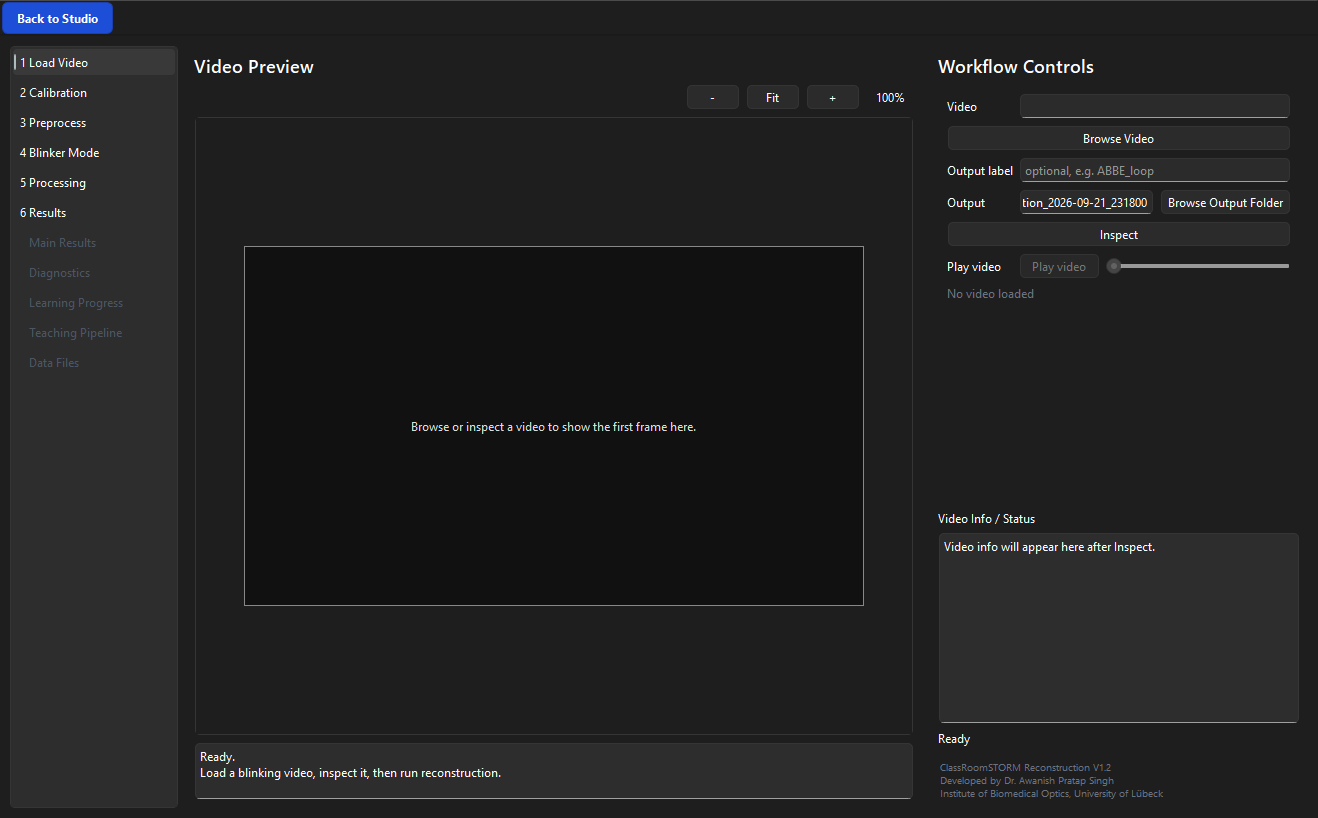
\includegraphics[width=\linewidth]{H6_reconstruction_load_crop}
  \caption{The SR Reconstruction window on the \ui{1 Load Video} page, showing
  the numbered step list, the video preview, and the workflow controls.}
  \label{fig:rc-load}
\end{figure}

\begin{figure}[htbp]
  \centering
  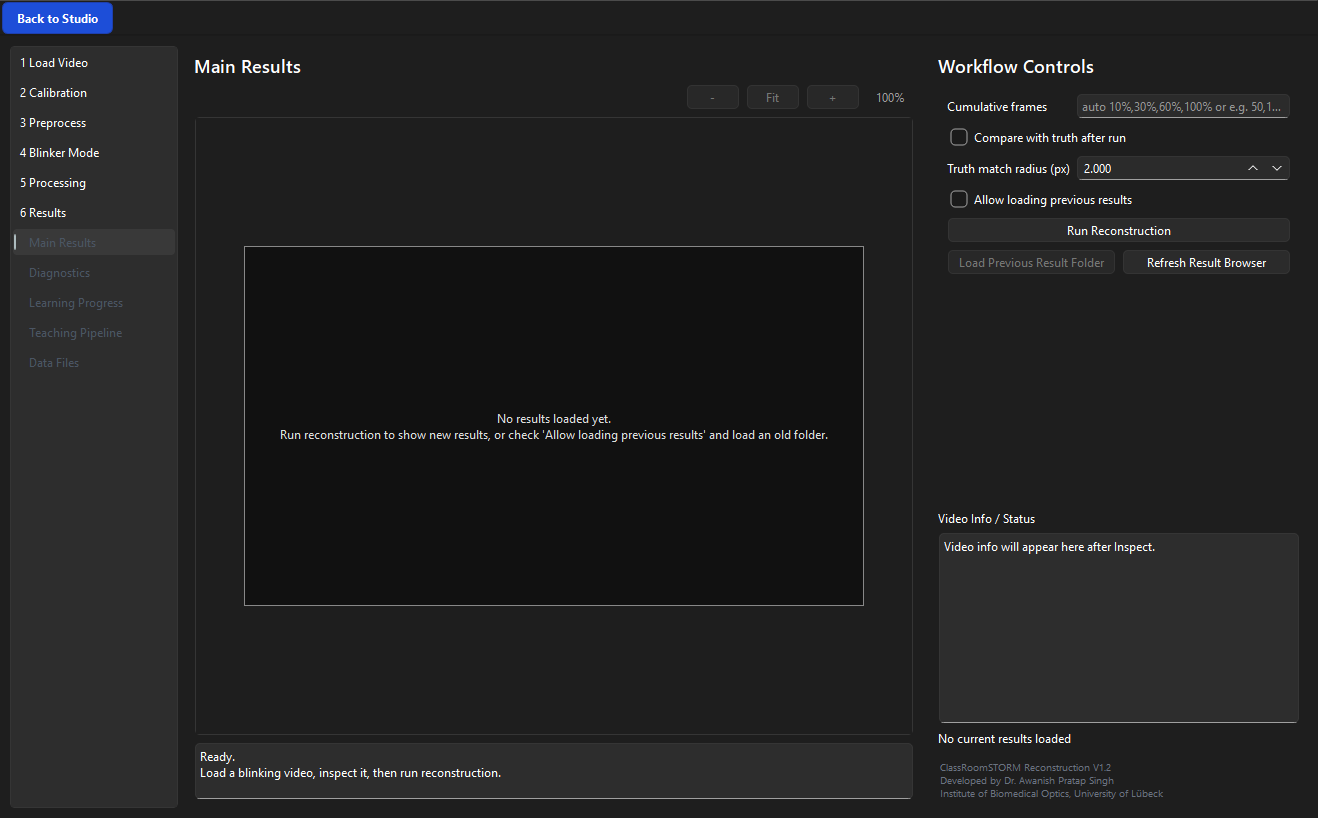
\includegraphics[width=\linewidth]{H7_results_browser}
  \caption{The SR Reconstruction \ui{Main Results} page. The result browser
  fills with images, plots, and data files once a reconstruction has run.}
  \label{fig:rc-results}
\end{figure}

% ======================================================================
\section{Linked Profile Viewer}
\label{sec:profiles}

The \ui{Linked Profiles} tab, in the \ui{Main Results} group, is a way to compare the raw and reconstructed images. It appears when a reconstruction has
produced both raw and reconstructed image data.

The viewer shows the \ui{Raw mean} image and the \ui{Reconstruction} image side
by side, with two line-profile plots beneath them. \textbf{Click anywhere on
either image} to place a crosshair; the plots update to show the intensity along
the row and the column through that point.

\begin{itemize}
  \item The \textcolor{red!70!black}{\textbf{red}} curve is the \ui{Raw mean} image, which appears as a wide, blurred bump.
  \item The \textcolor{blue!70!black}{\textbf{blue}} curve is the
        \ui{Reconstruction}, which displays positions using a fixed-width kernel.
\end{itemize}

The horizontal axis is the pixel coordinate; the vertical axis is normalized
intensity (each curve is scaled to a 0-1 range so the shapes can be compared
directly). Displayed peak width depends on the rendering kernel and normalization;
a narrow reconstruction peak alone is not a resolution measurement.

\begin{figure}[htbp]
  \centering
  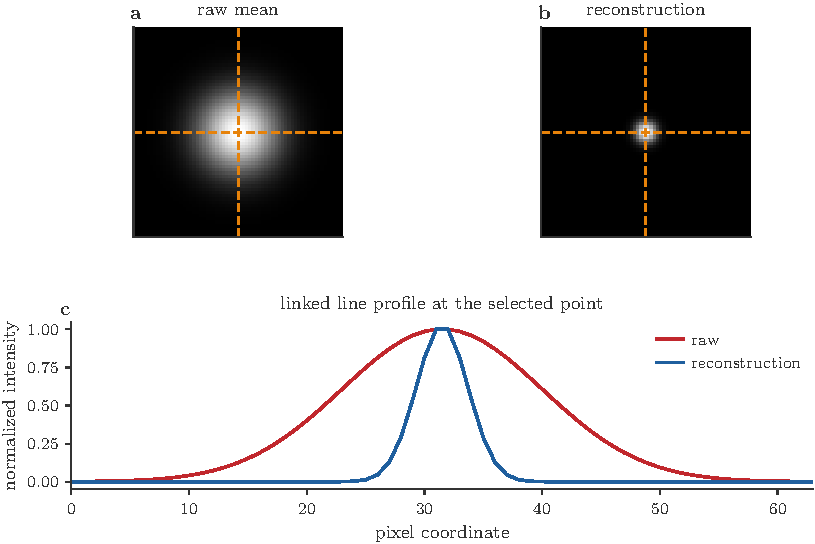
\includegraphics[width=\linewidth]{H8_linked_profile}
  \caption{Linked row profiles from the recorded two-source synthetic reconstruction. Dashed horizontal lines identify camera row 40; each profile is peak-normalized. A profile describes the displayed images and is not an independent resolution measurement.}
  \label{fig:profiles}
\end{figure}

% ======================================================================
\section{Reading Output Files and Diagnostic Figures}
\label{sec:reading}

\begin{description}[style=unboxed, leftmargin=0pt]
  \item[\ui{Raw Mean}] The arithmetic mean of all processed frames, forming a diffraction-limited, blurry image.
  \item[\ui{Super-Resolution}] The reconstructed image, built by accumulating
        all localizations.
  \item[\ui{Raw vs Super-Resolution}] The two images side by side.
  \item[\ui{Localization Scatter} / \ui{Density Map} / \ui{Raw Overlay}]
        Diagnostic plots: localization positions, their density, and their distribution over the raw image.
  \item[\ui{Learning Progress}] Cumulative reconstructions showing how the image
        sharpens as more frames are added.
  \item[\ui{Teaching Pipeline}] A step-by-step report (\file{pipeline\_report
        .html}) and pipeline diagrams.
  \item[\ui{Data Files}] The numerical results: \file{localizations.csv} and
        \file{summary.json}.
\end{description}

\begin{figure}[htbp]
  \centering
  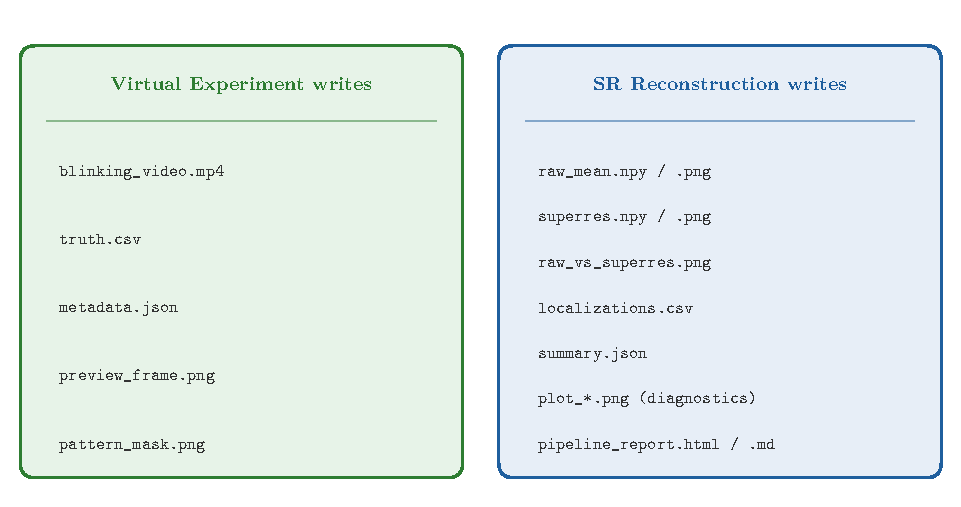
\includegraphics[width=\linewidth]{H9_output_map}
  \caption{Output roles for the virtual experiment and reconstruction workflows.}
  \label{fig:outputs}
\end{figure}

% ======================================================================
\section{Input and Output File Table}
\label{sec:files}
Table~\ref{tab:io} lists the files read and written by each workflow.

\begin{table}[htbp]
\centering\small
\begin{tabularx}{\linewidth}{@{}llX@{}}
\toprule
\textbf{Workflow} & \textbf{Direction} & \textbf{Files}\\
\midrule
Virtual Experiment & reads & a logo image (logo mode only)\\
Virtual Experiment & writes & \file{blinking\_video.mp4}, \file{truth.csv},
  \file{preview\_frame.png}, \file{pattern\_mask.png}, \file{metadata.json}\\
\midrule
SR Reconstruction & reads & a blinking video (MP4/AVI/MOV); optionally
  \file{truth.csv} for comparison\\
SR Reconstruction & writes & \file{localizations.csv};
  \file{raw\_mean.npy} and \file{raw\_mean.png};
  \file{superres.npy} and \file{superres.png};
  \file{raw\_vs\_superres.png}; \file{localization\_scatter.png};
  \file{plot\_density\_map.png}; \file{plot\_raw\_localization\_overlay.png};
  \file{plot\_cumulative\_reconstruction.png}; \file{summary.json};
  \file{pipeline\_report.md} / \file{.html}; pipeline diagram files\\
\bottomrule
\end{tabularx}
\caption{Files read and written by each workflow.}
\label{tab:io}
\end{table}

% ======================================================================
\section{Troubleshooting}
\label{sec:troubleshoot}

\begin{description}[style=unboxed, leftmargin=0pt]
  \item[Setup fails to download the packages.]
        This usually means that there is no internet access or that a restricted or proxy network prevents Python from verifying PyPI security certificates (a
        \texttt{CERTIFICATE\_VERIFY\_FAILED} error). Try an unrestricted network,
        ask your IT support how pip should reach PyPI, or use a package that
        includes an offline \file{wheels} folder.
  \item[Windows says Python was not found or opens the Microsoft Store.]
        Run \file{setup\_windows.bat} again and use its Python install option, or
        install Python 3.11, 3.12, or 3.13 from \url{https://www.python.org/}.
        If Windows keeps opening the Microsoft Store, disable the
        \file{python.exe} and \file{python3.exe} shortcuts in
        \ui{Settings > Apps > Advanced app settings > App execution aliases}.
  \item[The application will not start, or a ``ModuleNotFoundError'' appears.]
        The required packages are not installed. Run the setup script
        (\file{setup\_windows.bat} or \file{setup\_macos.command}) and wait for
        the \emph{Setup completed} message before launching again.
  \item[The launcher disappeared after I clicked a workflow.]
        This is expected. The launcher closes itself when a workflow opens. Use
        the \ui{Back to Studio} toolbar button at the top of the workflow window,
        or run the launch command again to get it back.
  \item[No bright spots are detected / the reconstruction is empty.]
        Check the contrast in the first video frame. Very dark or very noisy
        videos may have no clear spots. Try \texttt{multiple} blinker mode.
  \item[The reconstruction looks too sparse.]
        Use more frames, or (for a Virtual Experiment) increase
        \ui{Max blinkers/frame}.
  \item[A GPU backend seems no faster.]
        It probably fell back to the CPU. Check \file{summary.json}; install the
        optional GPU packages if you have an NVIDIA CUDA card.
  \item[Reconstruction fails immediately with a crop error.]
        \ui{Crop width}/\ui{Crop height} are zero. Inspect the video first to
        fill them, or untick \ui{Enable crop}.
  \item[The video will not load.]
        Make sure it is an MP4, AVI, or MOV file that OpenCV can read.
  \item[The \ui{Linked Profiles} tab is missing.]
        It appears only when a reconstruction has produced the raw and
        super-resolution data. Run a reconstruction first.
  \item[Truth comparison does nothing.]
        Make sure \file{truth.csv} is in the same folder as the video and that
        \ui{Compare with truth after run} is ticked.
  \item[A run is very slow.]
        Lower \ui{Max frames} for a test, or use \ui{Auto CPU}.
\end{description}

% ======================================================================
\section{Glossary}
\label{sec:glossary}

\begin{description}[style=unboxed, leftmargin=0pt, itemsep=2pt]
  \item[Blinker] A light source that switches on and off; it appears as a bright
        spot when on.
  \item[Localization] An estimate of the position of one bright spot's centre.
  \item[Centroid] The brightness-weighted average position of a spot's pixels;
        the method \app{} uses to localize spots.
  \item[Threshold] The brightness level above which pixels are treated as part
        of a spot.
  \item[Point-spread width ($\sigma$)] How wide a single point of light appears
        after blurring; the \ui{sigma\_px} control.
  \item[Reconstructed (super-resolution) image] The sharp image built by
        accumulating localizations.
  \item[Raw mean] The blurry arithmetic mean of the video frames.
  \item[Ground truth] The known, exact source positions, saved in
        \file{truth.csv}, used only to evaluate a reconstruction afterwards.
  \item[Frame] One image in the video.
  \item[Signal photons] The brightness of a blinker, set by \ui{Brightness}.
  \item[Background] A constant light level added to every pixel.
  \item[Read noise] Random camera-like noise added to each pixel.
  \item[Field of view / crop] The region of the video that is processed.
  \item[Pipeline report] The step-by-step teaching report produced after a run.
\end{description}

% ======================================================================
\Needspace{26\baselineskip}
\section{Instructor Notes}
\label{sec:instructors}

\paragraph{Short session (2-3 hours).} Use the Virtual Experiment only.
Students generate a dataset, reconstruct it, and explore the linked profiles. One useful question is: \emph{why} is the blue curve narrower than the red one?

\paragraph{Longer project (1-2 weeks).} Add a recorded video of physical blinking sources (for example, from a classroom optical setup or an LED source) and have
students compare reconstructions of simulated and real data.

\paragraph{Learning goals.}
\begin{itemize}
  \item Compare a raw (diffraction-limited) image with a localization-based
        reconstruction.
  \item Understand the truth-data rule: why the answer key is hidden until after
        reconstruction.
  \item Explore how blur width, noise, blinker density, and overlap affect the
        result.
  \item Treat physical calibration as optional; the core workflow uses pixel coordinates.
\end{itemize}

\paragraph{Suggested parameter sweeps.} Have students vary one setting at a time
and predict its effect before running the simulation: \ui{sigma\_px} (blur), \ui{Read noise},
\ui{Max blinkers/frame} (density and overlap), and \ui{Frames} (sampling). The
companion \emph{Theory} document gives the physics behind each of these.

\vfill
\noindent\rule{\linewidth}{0.4pt}\\[2pt]
{\footnotesize The science behind \app{} (diffraction, point-spread functions, blinking, localization, and precision) is explained in the
companion document \emph{\app{} Theory Notes}.}

\end{document}
